\documentclass[titlepage]{article}
\usepackage[margin=0.5in]{geometry}
\usepackage{graphicx}
\usepackage{minted}

\title{VLSI \\Assignment 5}
\author{Md Sahil\\BCSE IV\\Roll-001710501029}
\date{}

\begin{document}
    {\maketitle}

    \section{Describtion}
    \begin{itemize}
        \item 2 bit comparator
        \begin{itemize}
        \item Write a procedure for implementing 2-bit magnitude comparator.
        \item Write a test bench for 2-bit magnitude comparator
        \end{itemize}
    \item 4 bit comparator
        \begin{itemize}
            \item Write a procedure for implementing 4-bit magnitude comparator using 2-bit magnitude comparator.
            \item Write a test bench for 4-bit magnitude comparator
        \end{itemize}
    \item 8 bit comparator
        \begin{itemize}
            \item Write a procedure for implementing 8-bit magnitude comparator using 4-bit magnitude comparator.
            \item Write a test bench for 8-bit magnitude comparator.
            \item Write a procedure for implementing 8-bit magnitude comparator using 2-bit magnitude comparator.
            \item Implement 8-bit magnitude comparator by structural modelling.
        \end{itemize}
    \end{itemize}

    \section{Block Diagram} 
    \begin{figure}[!ht]
        \centering
        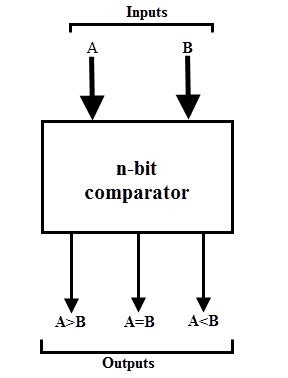
\includegraphics[width=7cm]{./figures/comparator_block_diagram.jpg}
        \caption{Decoder block diagram}
    \end{figure}


    \section{Truth Table}
    \begin{tabular}{| c | c | c |}
        \hline
        A(1 - 0) & B(1 - 0) & C(2 - 0)\\
        \hline
        00 & 00 & 010 \\
        00 & 01 & 001 \\
        00 & 10 & 001 \\
        00 & 11 & 001 \\
        01 & 00 & 100 \\
        01 & 01 & 010 \\
        01 & 10 & 001 \\
        01 & 11 & 001 \\
        10 & 00 & 100 \\
        10 & 01 & 100 \\
        10 & 10 & 010 \\
        10 & 11 & 001 \\
        11 & 00 & 100 \\
        11 & 01 & 100 \\
        11 & 10 & 100 \\
        11 & 11 & 010 \\
        \hline
    \end{tabular}
    \section{Circuit Diagram}
    \begin{figure}[!ht]
        \centering
        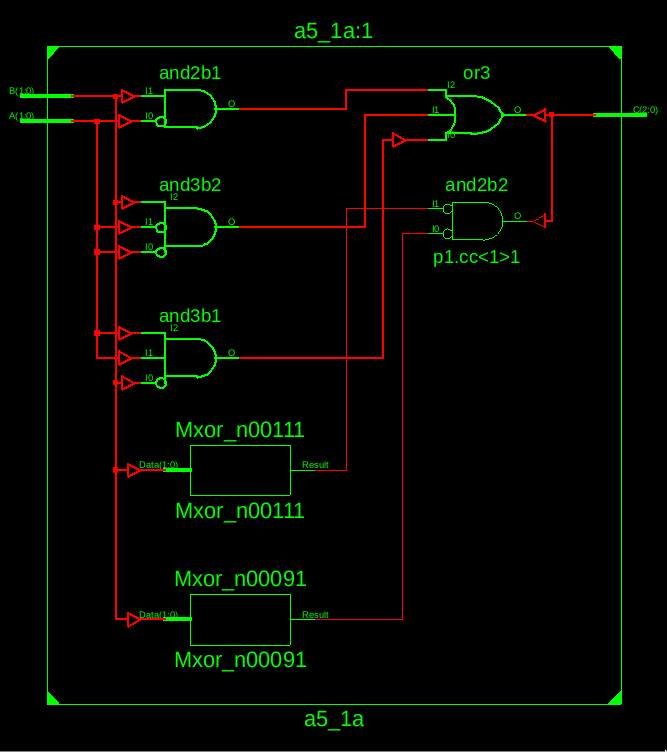
\includegraphics[width=12cm]{./figures/2bit_com.jpeg}
        \caption{2 bit comparator circuit diagram}
    \end{figure}
    \begin{figure}[!ht]
        \centering
        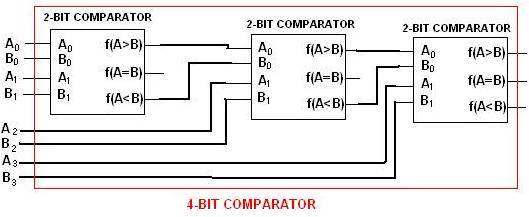
\includegraphics[width=12cm]{./figures/4bit.jpg}
        \caption{4 bit comparator using 2 bit comparators}
    \end{figure}
    \begin{figure}[!ht]
        \centering
        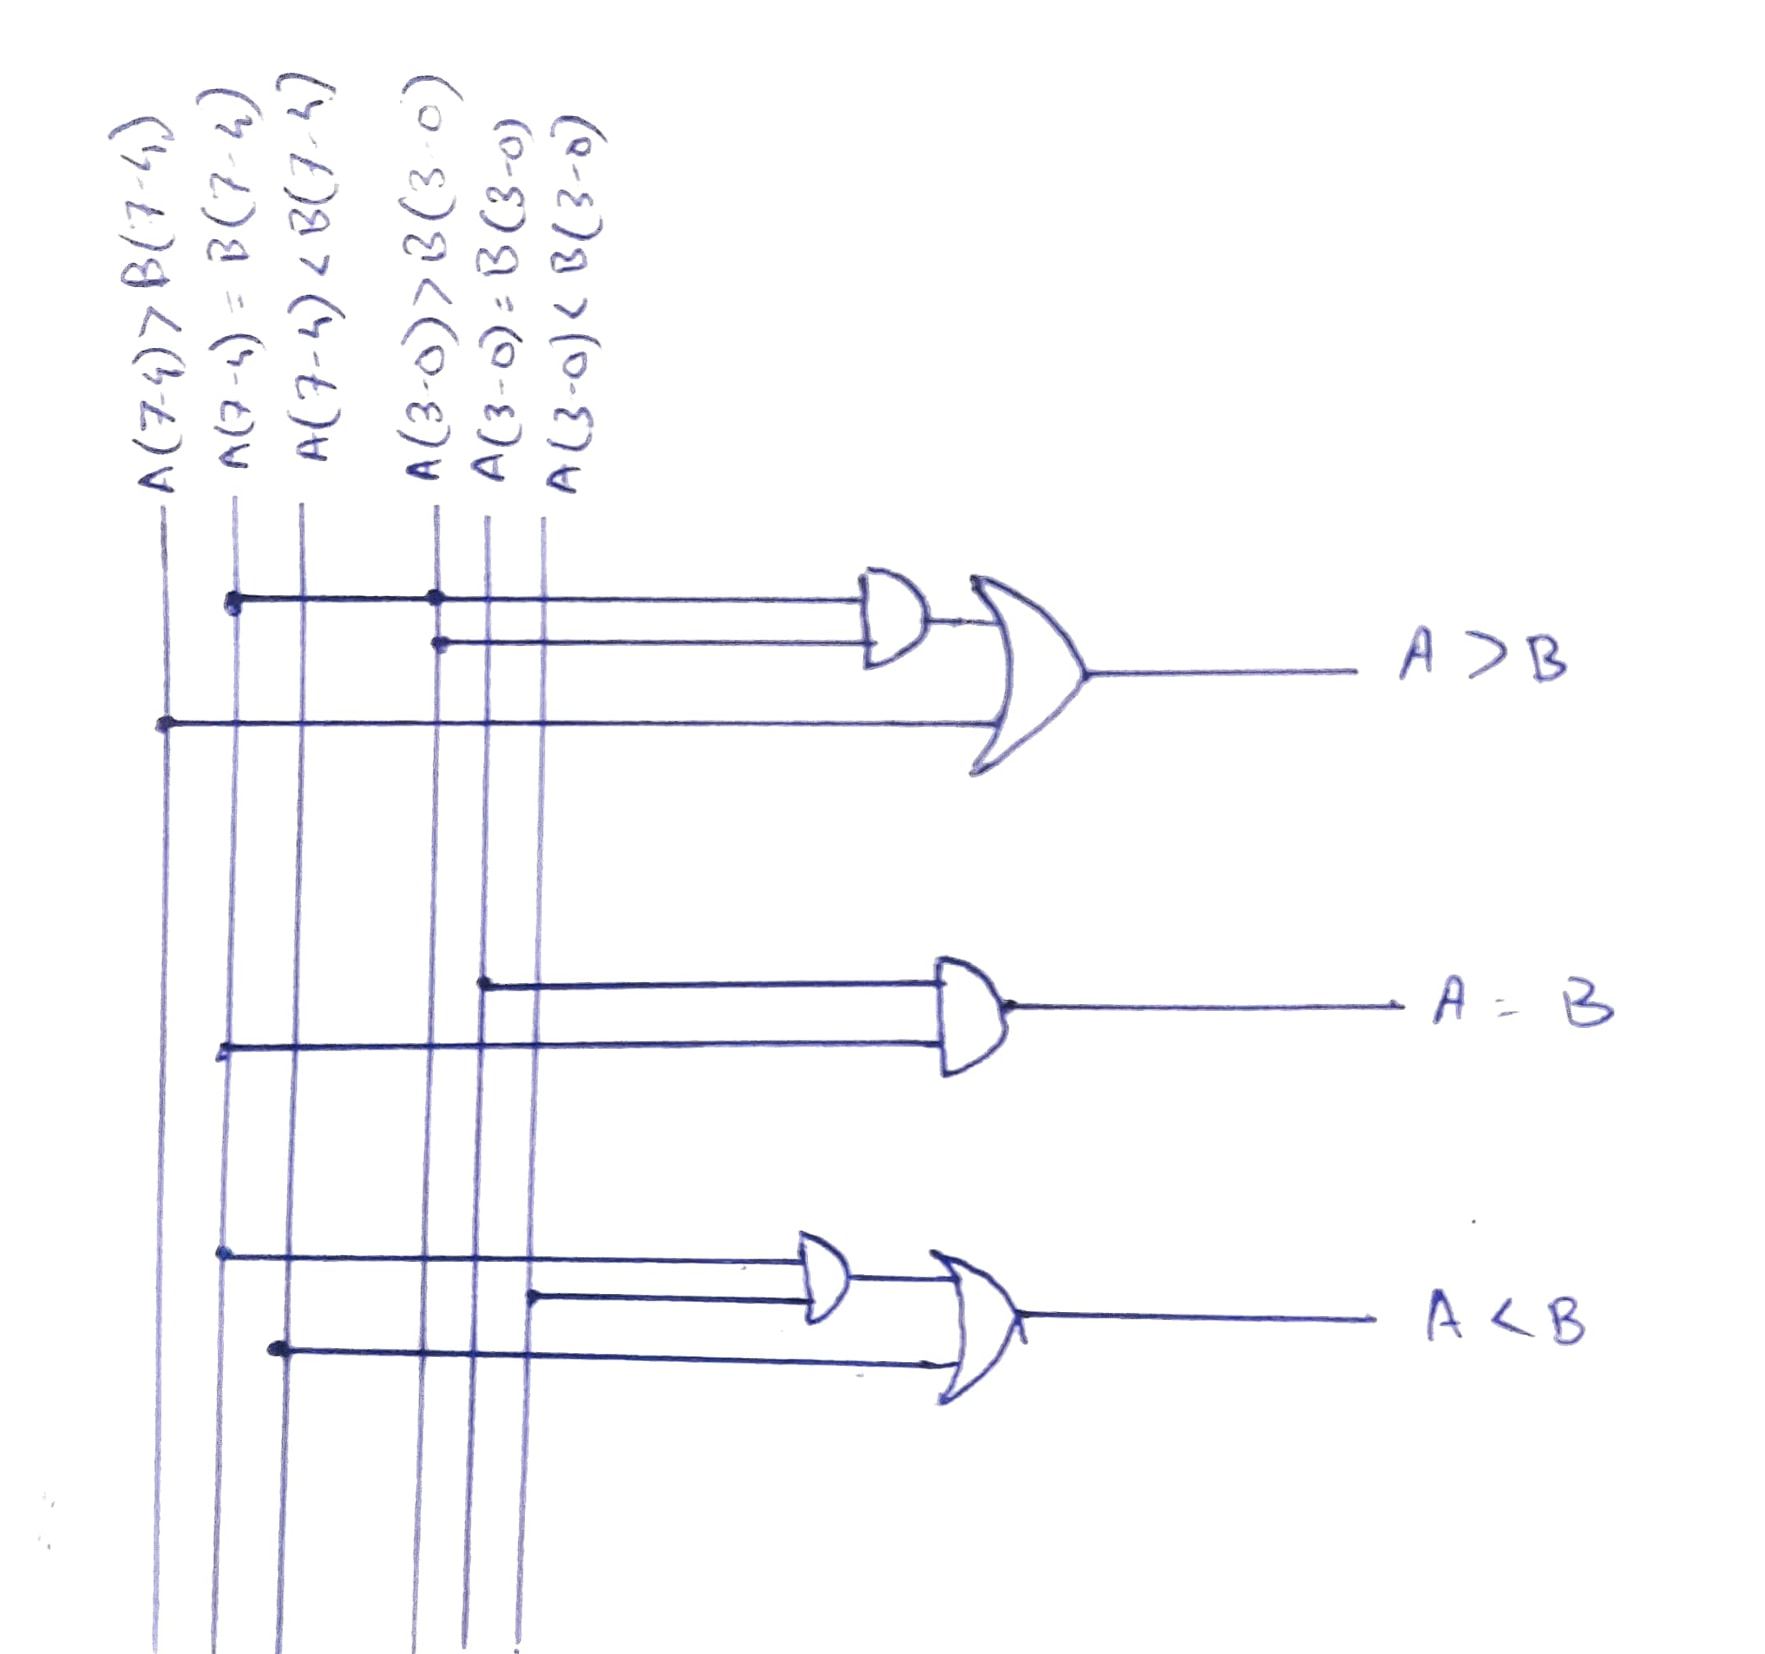
\includegraphics[width=12cm]{./figures/8bit_4bit.jpeg}
        \caption{8 bit comparator using 4 bit comparators}
    \end{figure}
    \begin{figure}[!ht]
        \centering
        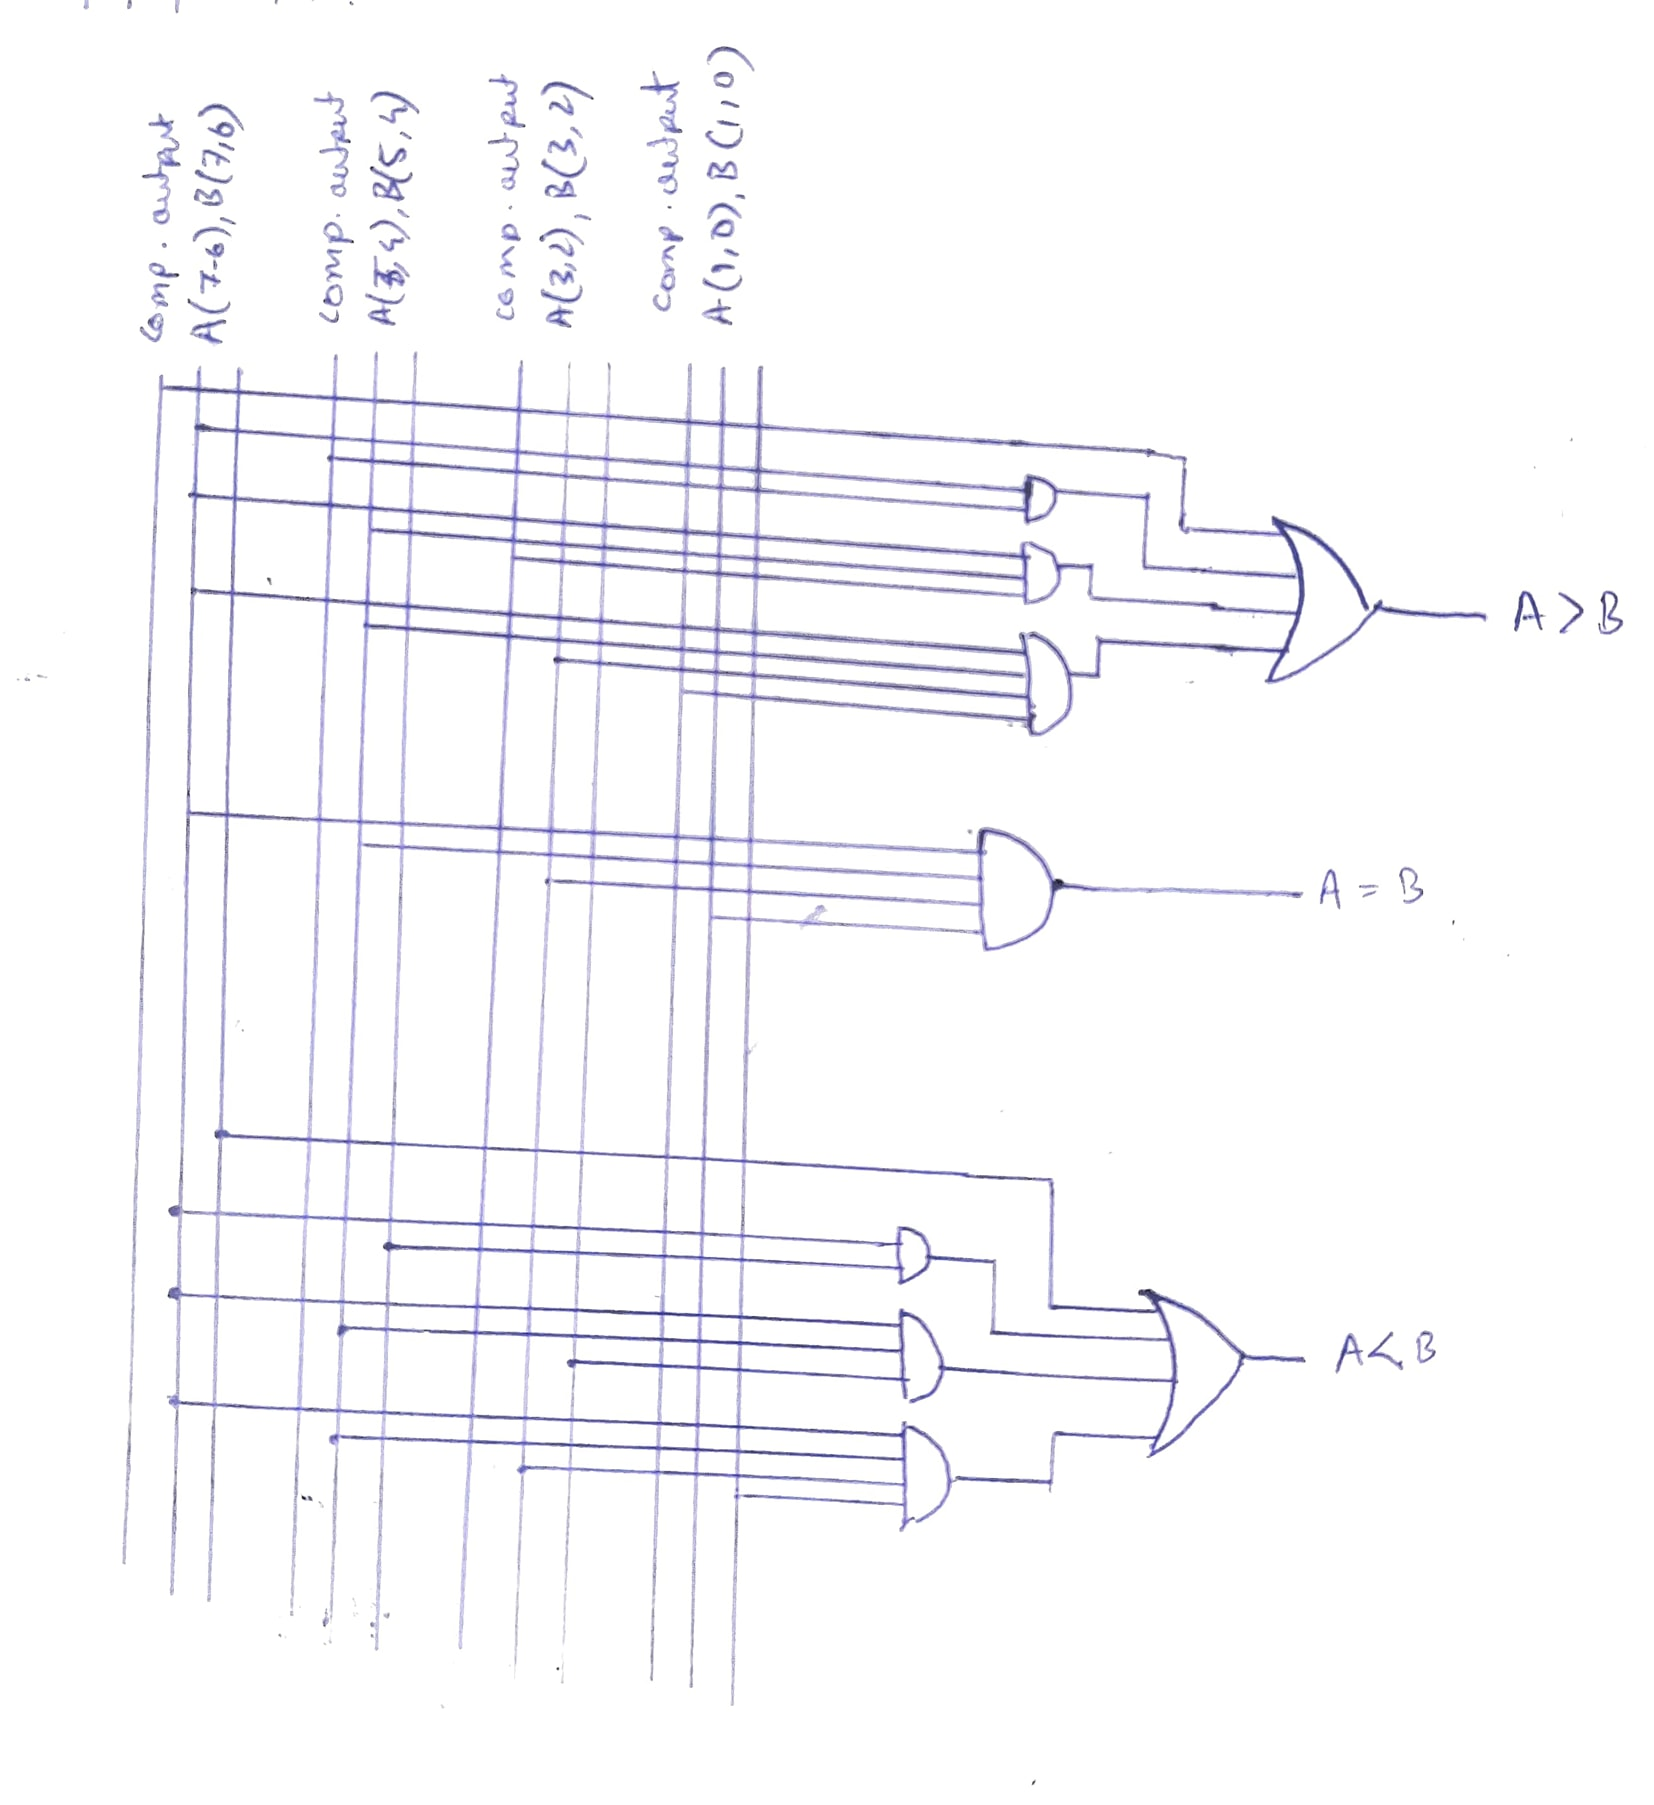
\includegraphics[width=12cm]{./figures/8bit_2bit.jpeg}
        \caption{8 bit comparator using 2 bit comparators}
    \end{figure}

    \section{Code for package}
    \inputminted{vhdl}{./codes/comparator_package.vhd}
    \section{Code for 2 bit comparator}
        \subsection{Module}
        \inputminted{vhdl}{./codes/a5_1a.vhd}
        \subsection{TestBench}
        \inputminted{vhdl}{./codes/tb_a5_1a.vhd}
        \subsection{Timing diagram}
        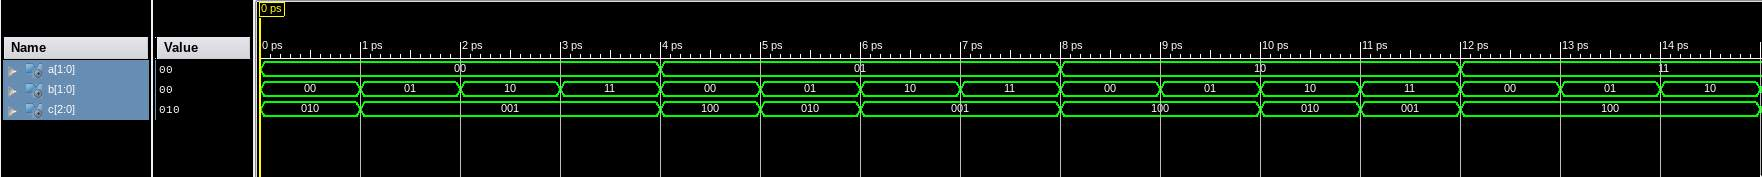
\includegraphics[width=19cm]{./figures/2bit_td.jpeg}
    \section{Code for 4 bit comparator using 2 bit comparator}
        \subsection{Module}
        \inputminted{vhdl}{./codes/a5_1b.vhd}
        \subsection{TestBench}
        \inputminted{vhdl}{./codes/tb_a5_1b.vhd}
        \subsection{Timing diagram}
        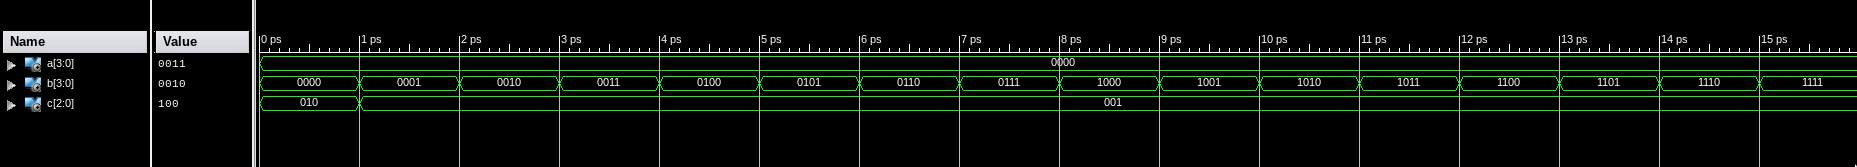
\includegraphics[width=19cm]{./figures/4bit_td.jpeg}
    \section{Code for 8 bit comparator}
        \subsection{Using 4 bit comparators}
        \inputminted{vhdl}{./codes/a5_3.vhd}
        \subsection{TestBench for 8 bit using 4 bit comparators}
        \inputminted{vhdl}{./codes/tb_a5_3.vhd}
        \subsection{Using 2 bit comparators}
        \inputminted{vhdl}{./codes/a4_4a.vhd}
        \subsection{TestBench for 8 bit using 2 bit comparators}
        \inputminted{vhdl}{./codes/tb_a4_4a.vhd}
        \subsection{Using Structural modelling}
        \inputminted{vhdl}{./codes/a5_4b.vhd}
        \subsection{TestBench for 8 bit using structural modelling}
        \inputminted{vhdl}{./codes/tb_a5_4b.vhd}
        \subsection{Timing diagram}
        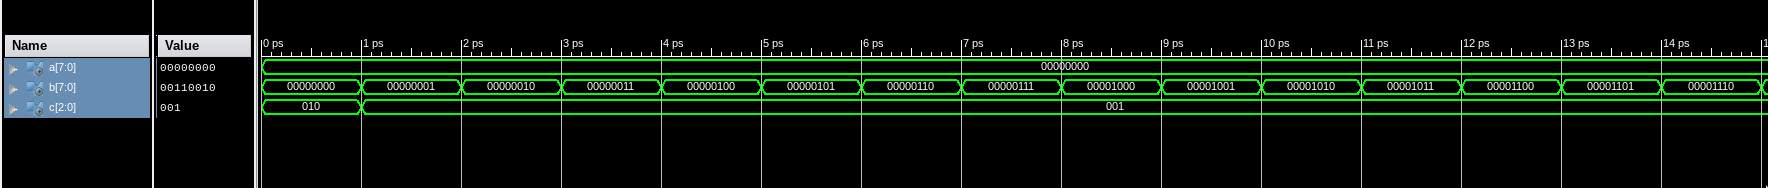
\includegraphics[width=19cm]{./figures/8bit_td.jpeg}

\end{document}
